			
						
					\chapter{Arhitektura i dizajn sustava}
			
			\begin{figure}[h]
				\centering
				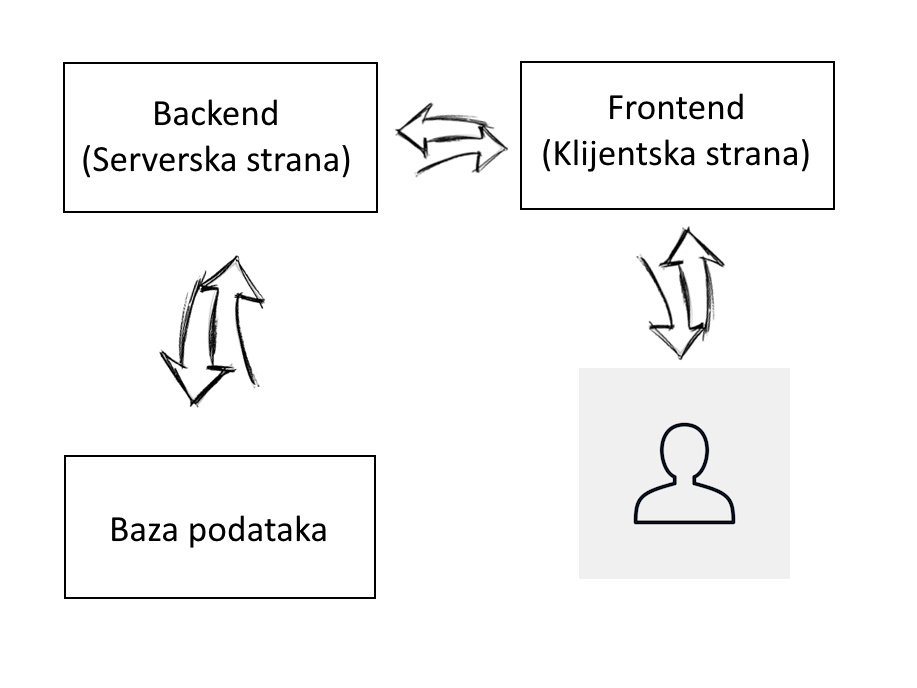
\includegraphics[width=0.8\textwidth]{slike/arhitektura-slika.jpg}
				\caption{Arhitektura sustava}
			\end{figure}
			
			{Korisnik aplikaciji pristupa putem web preglednika. Interakciju s aplikacijom ostvaruje preko korisničkog sučelja pomoću kojeg šalje zahtjeve web poslužitelju i prima odgovore.
				
				Programski jezik pomoću kojeg je ostvaren backend web aplikacije je C\#, a korišteni radni okvir je .NET. Frontend aplikacije ostvaren je programskim jezikom
				TypeScript i radnim okvirom Angular. Za razvojno okruženje backend-a odabran je Visual Studio, a frontend-a Visual Studio Code.
				
				.NET je radni okvir namijenjen stvaranju mikroservisa. Mikroservisi su arhitektura razvoja softvera koja podrazumijeva izgradnju aplikacije pomoću niza malih, nezavisnih servisa. Svaki mikroservis obavlja određeni posao i može komunicirati s drugim mikroservisima preko standardiziranih protokola. Primjena mikroservisne arhitekture u razvoju web aplikacija omogućuje agilniji pristup razvoju, povećava skalabilnost, pojednostavljuje održavanje i prilagodljivost sustava promjenama. Svaki mikroservis može se smatrati zasebnim servisom unutar web aplikacije, obavljajući specifične funkcionalnosti, poput autentifikacije, upravljanja korisnicima, poslovnih logika, itd.
				
				Arhitektura sustava temelji se na MVC (Model-View-Controller) konceptu. MVC koncept predstavlja arhitekturni obrazac koji je podržan od strane .NET radnog okvira, pružajući gotove predloške koji značajno olakšavaju razvoj web aplikacija.
				
				MVC koncept omogućuje nezavisan razvoj pojedinih dijelova aplikacije, što rezultira jednostavnijim ispitivanjem i olakšanim dodavanjem novih svojstava u sustav. Takav pristup razdvaja sustav na tri ključna dijela:
				
				\begin{itemize}
					\item \textbf{Model:} Središnja komponenta sustava koja predstavlja dinamičke strukture podataka neovisne o korisničkom sučelju. Model izravno upravlja podacima, logikom i pravilima aplikacije. Također, prima ulazne podatke od Controllera.
					
					\item \textbf{View:} Odgovoran je za prikaz podataka, poput grafa ili tabličnog prikaza. View omogućuje različite prikaze istih informacija, poput grafičkog ili tabličnog prikaza podataka.
					
					\item \textbf{Controller:} Prima ulaze od korisnika i prilagođava ih za prosljeđivanje Modelu ili Viewu. Controller upravlja korisničkim zahtjevima i temeljem njih izvodi daljnju interakciju s ostalim elementima sustava. Osim posredovanja između Modela i Viewa, Controller igra ključnu ulogu u usmjeravanju tijeka aplikacije.
				\end{itemize}
				
				Ovaj trojni raspored omogućuje jasno definiranje odgovornosti svake komponente, čime se postiže modularnost sustava. Model upravlja podacima, View se brine o prezentaciji, dok Controller koordinira interakcijom između njih. Ovaj pristup često rezultira čistim, lako održivim kodom i olakšava daljnji razvoj aplikacije.
				\\
				\\
				Web aplikaciju čine tri osnovna dijela:
				\begin{itemize}
					\item \textbf{Frontend}
					\item \textbf{Backend}
					\item \textbf{Baza podataka}
				\end{itemize}
				
				Frontend se sastoji od komponenata i logike. Istu komponentu je moguće koristiti za različite namjene (engl. reusability). Angular koristi koncept komponenata i servisa koji omogućuje ponovnu upotrebu koda.  Angular koristi svojstva poput Dependency Injection i Change Detection za poboljšanje performansi. Struktura je ostvarena povezivanjem različitih komponenata unutar hijerarhijske strukture.\\
				
				Backend je ključna komponenta web aplikacije, sastavljena od sljedećih dijelova:
				
				\begin{itemize}
					\item \textbf{Programsko sučelje za reprezentacijski prijenos stanja (REST API):}
					Controller je odgovoran za obradu zahtjeva koji dolaze od korisnika ili drugih dijelova aplikacije. On prima HTTP zahtjeve, interpretira ih, te ih proslijeđuje odgovarajućim dijelovima aplikacije. Nakon obrade zahtjeva, Controller šalje odgovor korisniku, koji se sastoji od statusnog koda, tijela poruke i zaglavlja. Sadržaj u tijelu poruke predstavlja informacije koje korisnik konzumira nakon što su prikazane u web pregledniku.
					
					\item \textbf{Sloj poslovne logike (Service):}
					Service je odvojeni sloj koji sadrži poslovnu logiku aplikacije. Ovdje se obrađuju i provjeravaju podaci, izvršavaju poslovne operacije te se komunicira s ostalim dijelovima sustava. Service često služi kao posrednik između Controllera i Repository sloja. Komunikaciju sa slojem poslovne logike Controller ostvaruje pomoću umetanja ovisnosti (dependency injection). Dependency injection je obrazac prema kojemu se u određeni objekt/funkciju umeće neki drugi objekt/funkcija na koji se prvobitno spomenuti objekt/funkcija oslanja.
					
					\item \textbf{Sloj za pristup bazi podataka (Repository):}
					Repository je odgovoran za komunikaciju s bazom podataka. Ovaj sloj omogućuje izvođenje operacija poput čitanja, pisanja, brisanja i ažuriranja podataka u bazi. Koristi se SQL upitima ili ORM (Object-Relational Mapping) tehnikama za pretvaranje podataka iz relacijske baze podataka u objekte koji se koriste unutar aplikacije. Repository omogućuje komunikaciju s bazom podataka pomoću SQL-a. Objekti iz relacijske baze podataka pretvaraju se u objekte programskog jezika Java pomoću tehnike ORM.
					
				\end{itemize}
				
				Ova trostruka podjela omogućuje jasnu strukturu i odvajanje odgovornosti unutar backend-a, čineći ga modularnim i lakšim za održavanje.
				
				
			}
			
			
			
			
			
			
			
			
			\section{Baza podataka}
			
			
			
			{
				Baza podataka za aplikaciju implementirana je kao relacijska baza podataka, gdje se podaci pohranjuju u obliku redaka ili n-torki te stupaca ili atributa koji zajedno čine tablicu. Ovaj pristup omogućuje strukturiranu organizaciju podataka, gdje svaka tablica predstavlja određenu vrstu informacija, a svaki redak u tablici predstavlja konkretan zapis ili entitet. Relacijski model olakšava učinkovito upravljanje podacima, omogućuje jednostavno pretraživanje i izvođenje kompleksnih upita nad podacima, što čini bazu podataka temeljem za pouzdano čuvanje i manipulaciju informacijama u aplikaciji.}
			
			\subsection{Opis tablica}
			
			
			{
				Glavna komponenta baze je tablica User, koja se puni osobnim podacima unesenim pri registraciji korisnika u sustav. Svakom novom korisniku dodjeljuje se primarni ključ, unikatni identifikacijski broj pomoću kojeg se korisnici u bazi podataka međusobno razlikuju. Budući da korisnik može biti primatelj usluge, davatelj usluge i menadžer usluge, postoji atribut roleId koji ovisno o broju označava ulogu korisnika u sustavu. Ako je korisnik menadžer, onda je povezan na tablicu Manager preko stranog ključa userId. Tablica Manager dodatno sadrži atribut confirmedByAdmin koji opisuje je li menadžer potvrđen od strane administratora aplikacije. Kako bi korisnik opće rezervirao parkirno mjesto, postoji tablica Parking koja sadrži svoj unikatni id, id vlasnika. Svako parkiralište ima n parkirališnih mjesta koja su opisana u tablici ParkingPlace sa stranim ključem na id parkirališta u čijem su vlasništvu, te tip mjesta uz cijenu i pokazatelj zauzetosti. U sustavu baze podataka također postoji tablica Vehicle koja opisuje vozilo. Vozilo ima strani ključ na id vlasnika, te vlastiti id i naziv. Kako bi sustav rezervacija funkcionirao, postoji tablica Reservation koja povezuje korisnika, parking, parkirno mjesto, vozilo te vrijeme same rezervacije. Svaki korisnik ima svoj novčanik opisan tablicom Wallet sa stranim ključem na korisnika i količinom novca kao atributom. Na samom kraju postoji tablica Transaction koja prati uplate i isplate u sustavu. 
			}
			
			
			\begin{longtblr}[
				label=none,
				entry=none
				]{
					width = \textwidth,
					colspec={|X[6,l]|X[6, l]|X[20, l]|}, 
					rowhead = 1,
				} %definicija širine tablice, širine stupaca, poravnanje i broja redaka naslova tablice
				\hline \SetCell[c=3]{c}{\textbf{USER}}	 \\ \hline[3pt]
				\SetCell{LightGreen} user ID	& INT & jedinstveni identifikator korisnika  	\\ \hline 
				username	& VARCHAR & korisničko ime  	\\ \hline 
				password & VARCHAR & hash lozinke  \\ \hline 
				name & VARCHAR	& ime korisnika 		\\ \hline 
				surname & VARCHAR	& prezime korisnika 		\\ \hline 
				IBAN & VARCHAR(34)	& IBAN korisnika koji se koristi prilikom plaćanja 		\\ \hline 
				email & VARCHAR	& email korisnika		\\ \hline 
				is email confirmed  & BOOLEAN	& potvrda je li korisnik potvrdio svoj račun preko mail-a 		\\ \hline 
				role id & INT	& broj korisnikove uloge u sustavu \\ \hline 
				id image path & VARCHAR	& fotografija osobne iskaznice korisnika 		\\ \hline 
			\end{longtblr}
			
			\begin{longtblr}[
				label=none,
				entry=none
				]{
					width = \textwidth,
					colspec={|X[6,l]|X[6, l]|X[20, l]|}, 
					rowhead = 1,
				} %definicija širine tablice, širine stupaca, poravnanje i broja redaka naslova tablice
				\hline \SetCell[c=3]{c}{\textbf{MANAGER}}	 \\ \hline[3pt]
				\SetCell{LightBlue}user ID & INT	&  	jedinstveni identifikator korisnika koji je menadžer parkinga, strani ključ  na user ID user tablice	\\ \hline
				confirmed by admin 	& BOOLEAN & vrijednost je li korisnik potvrđen od strane administratora da je menadžer  	\\ \hline 
			\end{longtblr}
			
			\begin{longtblr}[
				label=none,
				entry=none
				]{
					width = \textwidth,
					colspec={|X[6,l]|X[6, l]|X[20, l]|}, 
					rowhead = 1,
				} %definicija širine tablice, širine stupaca, poravnanje i broja redaka naslova tablice
				\hline \SetCell[c=3]{c}{\textbf{PARKING}}	 \\ \hline[3pt]
				\SetCell{LightGreen} parking ID	& INT & jedinstveni identifikator parkinga  	\\ \hline 
				\SetCell{LightBlue} owner ID & INT & ID na korisnika vlasnika parkinga, strani ključ	\\ \hline 
				parking name & VARCHAR	& ime parkinga 		\\ \hline 
				parking description & VARCHAR	& opis parkinga, koliko ima mjesta, lokacija, je li natkriven, je li osvijetljen...		\\ \hline 
				parking photo & VARCHAR	& fotografija parkinga \\ \hline
			\end{longtblr}
			
			\begin{longtblr}[
				label=none,
				entry=none
				]{
					width = \textwidth,
					colspec={|X[6,l]|X[6, l]|X[20, l]|}, 
					rowhead = 1,
				} %definicija širine tablice, širine stupaca, poravnanje i broja redaka naslova tablice
				\hline \SetCell[c=3]{c}{\textbf{PARKING SPACE}}	 \\ \hline[3pt]
				\SetCell{LightGreen} parking space ID	& INT & jedinstveni identifikator parkirnog mjesta  	\\ \hline 
				\SetCell{LightBlue} parking ID & INT & ID na parking u čijem je vlasništvu odabrano parkirno mjesto, strani ključ	\\ \hline 
				\SetCell{LightBlue} type & INT & id vozila ciji tip odgovara odabranom parkirnom mjestu (npr: automobil, bicikl...), strani ključ	\\ \hline 
				status & ID	& status zauzetosti parkinga, vrsta podatka je integer jer je s brojem označen status parkinga	\\ \hline 
				latitude & INT	& brojčana vrijednost fizičke širine parkinga, u metrima	\\ \hline 
				longitude & INT	& brojčana vrijednost fizičke duljine parkinga, u metrima	\\ \hline 
				price & INT	& cijena parkirnog mjesta, po satu \\ \hline
			\end{longtblr}
			
			\begin{longtblr}[
				label=none,
				entry=none
				]{
					width = \textwidth,
					colspec={|X[6,l]|X[6, l]|X[20, l]|}, 
					rowhead = 1,
				} %definicija širine tablice, širine stupaca, poravnanje i broja redaka naslova tablice
				\hline \SetCell[c=3]{c}{\textbf{VEHICLE}}	 \\ \hline[3pt]
				\SetCell{LightGreen} vehicle ID	& INT & jedinstveni identifikator vozila 	\\ \hline 
				vehicle name & VARCHAR & ime vozila \\ \hline 
			\end{longtblr}
			
			\begin{longtblr}[
				label=none,
				entry=none
				]{
					width = \textwidth,
					colspec={|X[6,l]|X[6, l]|X[20, l]|}, 
					rowhead = 1,
				} %definicija širine tablice, širine stupaca, poravnanje i broja redaka naslova tablice
				\hline \SetCell[c=3]{c}{\textbf{RESERVATION}}	 \\ \hline[3pt]
				\SetCell{LightGreen} reservation ID	& INT & jedinstveni identifikator rezervacije  	\\ \hline 
				\SetCell{LightBlue} user ID & INT & ID na korisnika koji je napravio rezervaciju, strani ključ	\\ \hline 
				reservation date & DATETIME & datum i vrijeme rezervacije	\\ \hline 
				duration & ID	& vremenska duljina rezervacije, u satima	\\ \hline 
				\SetCell{LightBlue}vehicle type & INT	& tip vozila na čije ime glasi rezervacija, strani ključ na tablicu vehicle	\\ \hline 
				\SetCell{LightBlue} parking space id & INT	& jedinstveni identifikator koje je točno parkirno mjesto rezervirano, strani ključ	\\ \hline 
				repeating & BOOLEAN	& vrijednost koja pokazuje treba li se rezervacija periodički ponavljati (na dnevnoj, tjednoj ili mjesečnoj razini...) \\ \hline
			\end{longtblr}
			
			\begin{longtblr}[
				label=none,
				entry=none
				]{
					width = \textwidth,
					colspec={|X[6,l]|X[6, l]|X[20, l]|}, 
					rowhead = 1,
				} %definicija širine tablice, širine stupaca, poravnanje i broja redaka naslova tablice
				\hline \SetCell[c=3]{c}{\textbf{TRANSACTION}}	 \\ \hline[3pt]
				\SetCell{LightGreen} transaction ID	& INT & jedinstveni identifikator transakcije 	\\ \hline 
				\SetCell{LightBlue} user ID	& INT & ID na korisnika koji je obavio transakciju, strani ključ 	\\ \hline 
				type & INT & tip transakcije \\ \hline 
				amount & FLOAT & količina novca koji je prošao kroz transakciju \\ \hline 
			\end{longtblr}
			
			\begin{longtblr}[
				label=none,
				entry=none
				]{
					width = \textwidth,
					colspec={|X[6,l]|X[6, l]|X[20, l]|}, 
					rowhead = 1,
				} %definicija širine tablice, širine stupaca, poravnanje i broja redaka naslova tablice
				\hline \SetCell[c=3]{c}{\textbf{WALLET}}	 \\ \hline[3pt]
				\SetCell{LightGreen} wallet ID	& INT & jedinstveni identifikator novčanika 	\\ \hline 
				\SetCell{LightBlue} user ID	& INT & ID na korisnika u čijem je vlasniku virtualni novčanik, strani ključ 	\\ \hline 
				balance & FLOAT & količina novca koji se nalazi u novčaniku \\ \hline 
			\end{longtblr}
			
			
			
			\subsection{Dijagram baze podataka}
			
			\begin{figure}[h]
				\centering
				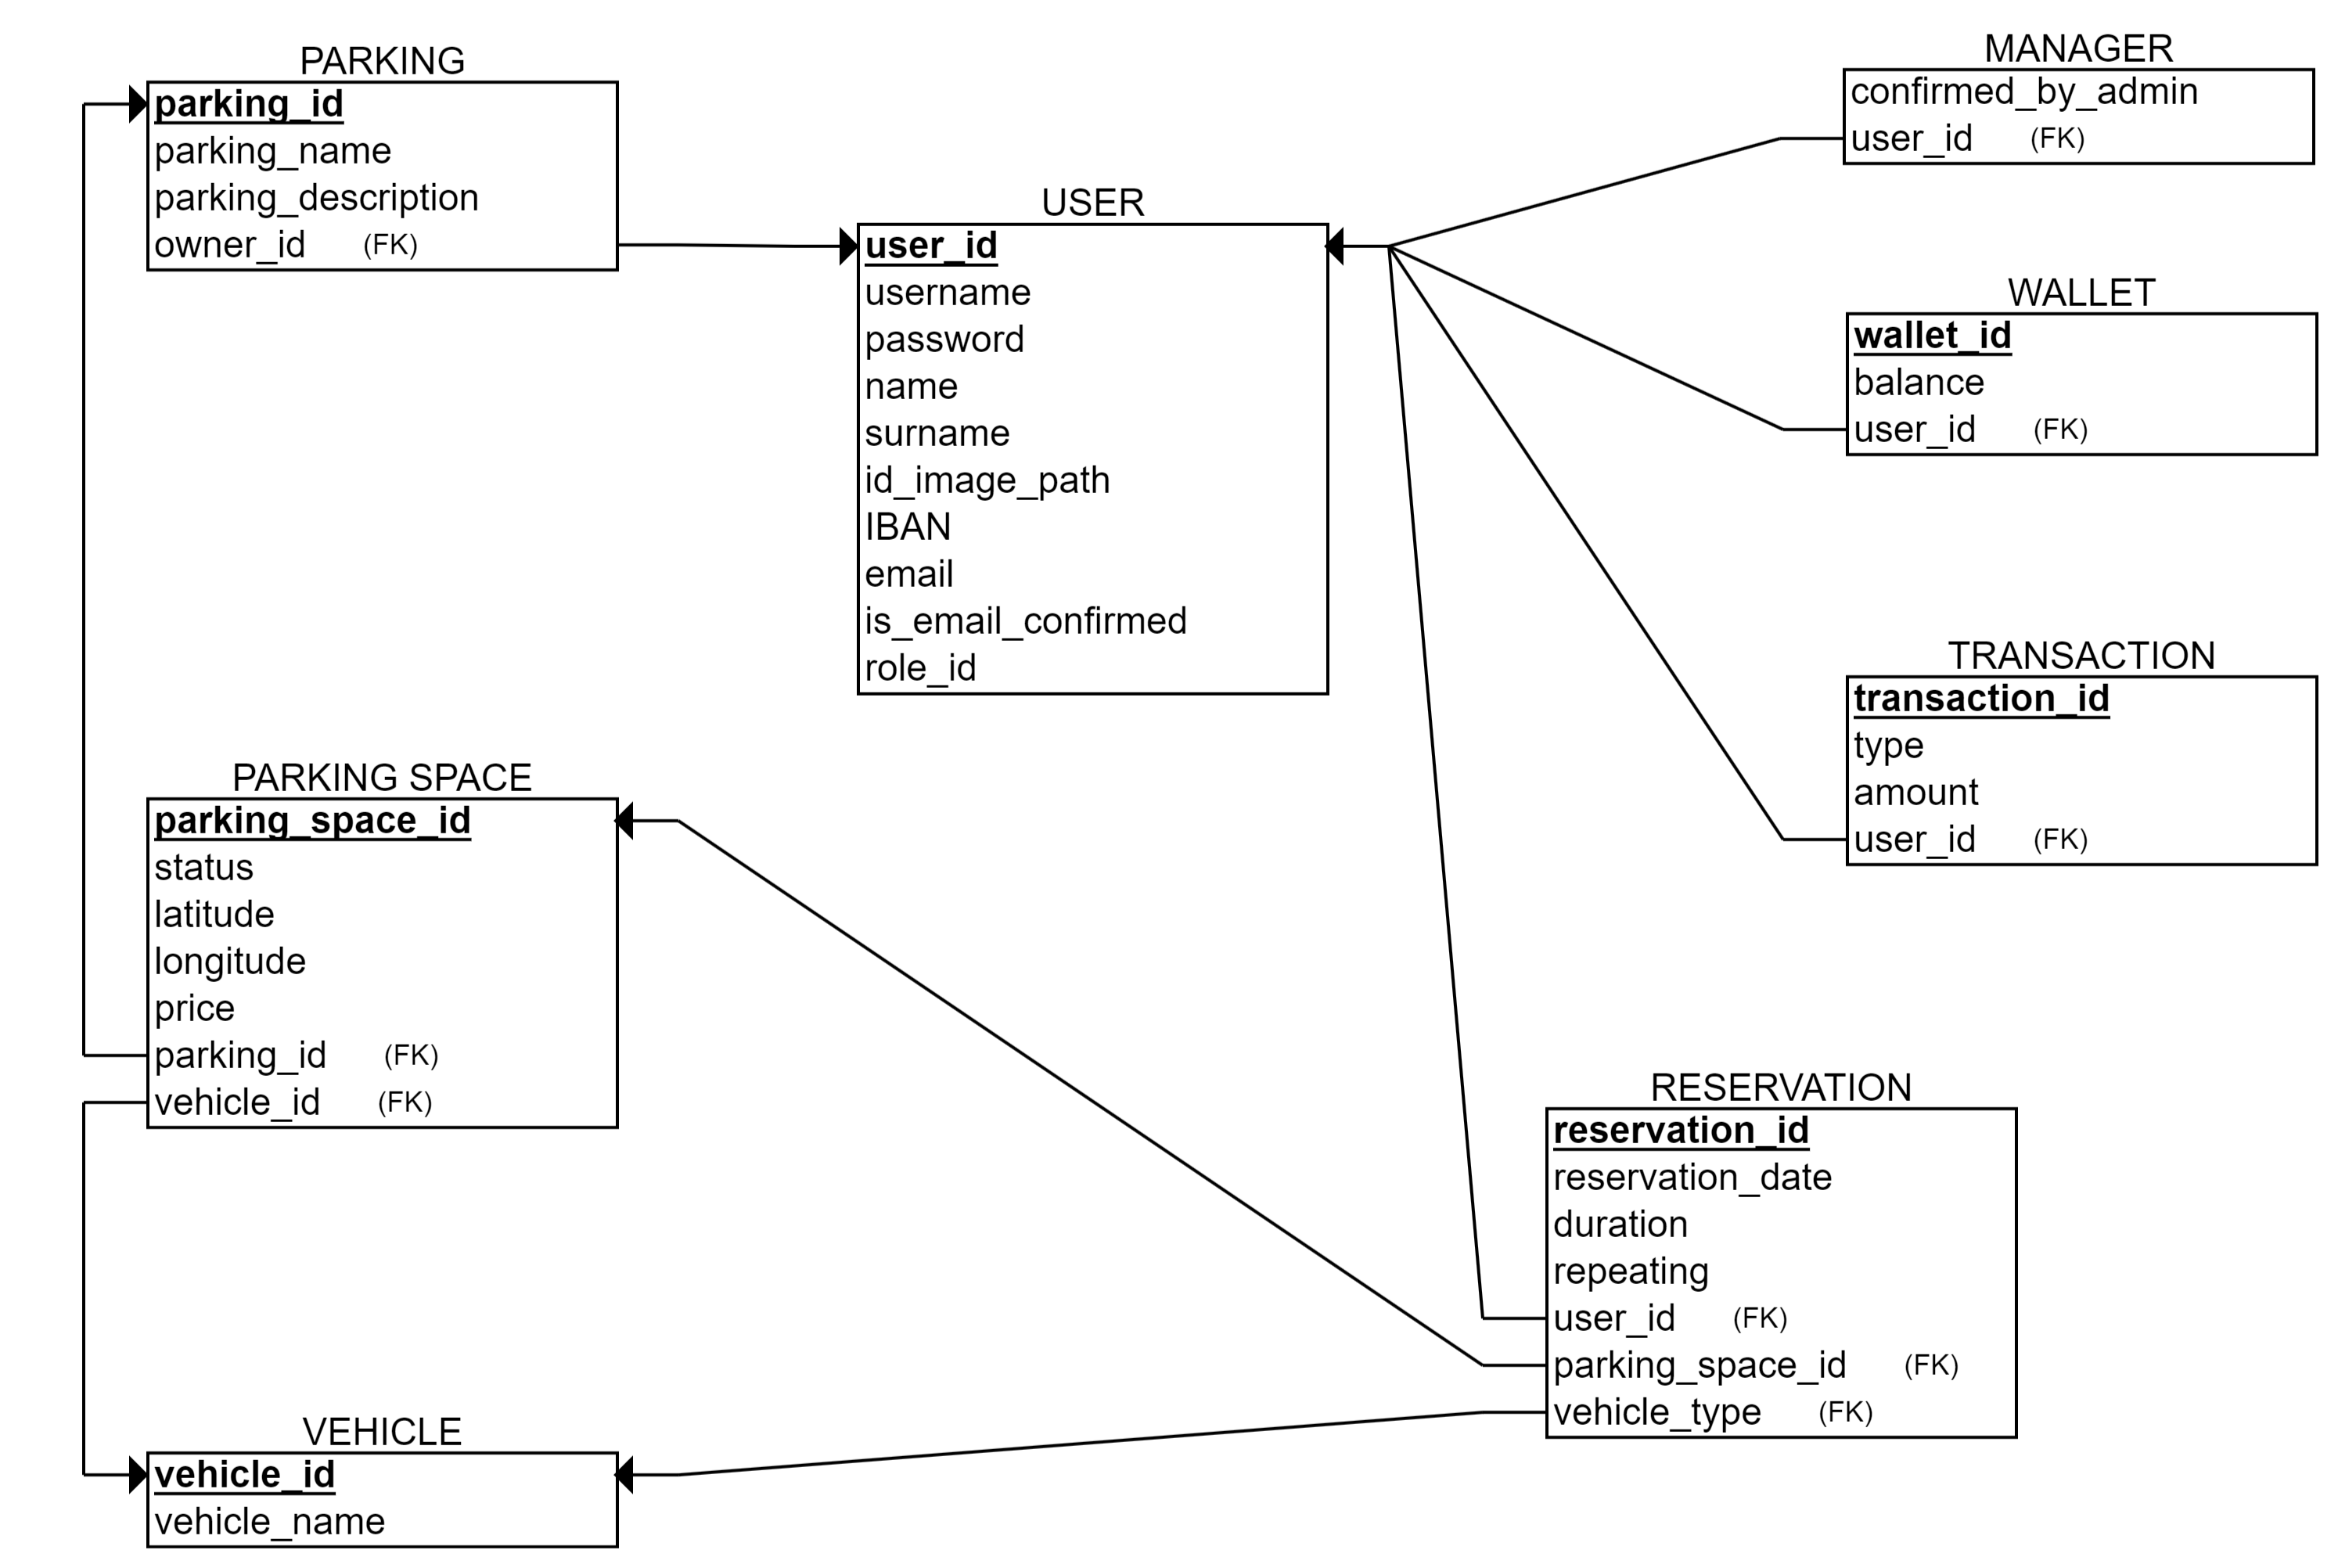
\includegraphics[width=0.8\textwidth]{slike/baza-slika.png}
				\caption{ER dijagram baze podataka}
			\end{figure}
			
			
			\section{Dijagram razreda} 
			
			{ Na slikama su prikazani razredi („Class“) koji su korišteni za implementaciju backend-a. Na slici \ref{fig:controllers} su prikazani razredi koji nasljeđuju Controller razred. Sve funkcije implementirane u Controller razredu vraćaju IActionResult (podatke i odgovarajući kod). Također, sve funkcije ne komuniciraju direktno s bazom podataka nego pozivaju funkcije iz određenih servisa koji imaju implementiranu tu funkcionalnost. Funkcije u kontrolerima kao parametre primaju odgovarajući model. }
			
			\begin{figure}[h]
				\centering
				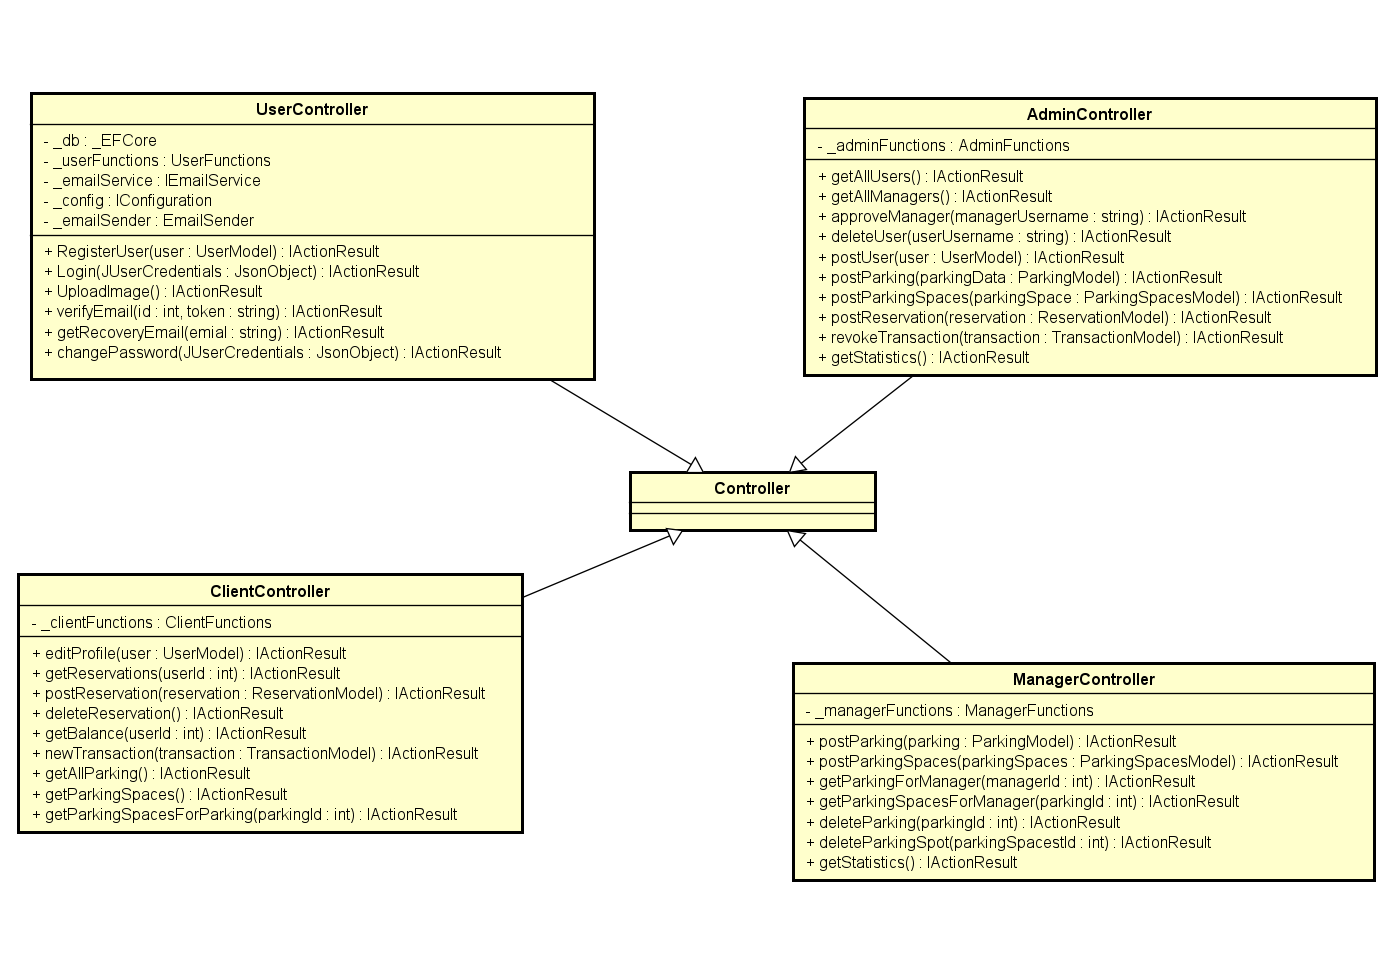
\includegraphics[width=\textwidth,keepaspectratio]{slike/progi4_1.png}
				\caption{dio Controllers}
				\label{fig:controllers}
			\end{figure}
			\pagebreak
			
			{Modeli razreda odražavaju strukturu baze podataka unutar aplikacije. Metode implementirane unutar tih razreda izravno komuniciraju s bazom podataka kako bi dobile tražene informacije. Razred User predstavlja generičnog korisnika aplikacije koji se može registrirati. Na taj razred referira se razred Manager (jer je svaki Manager ujedno i User).}
			
			\begin{figure}[h]
				\centering
				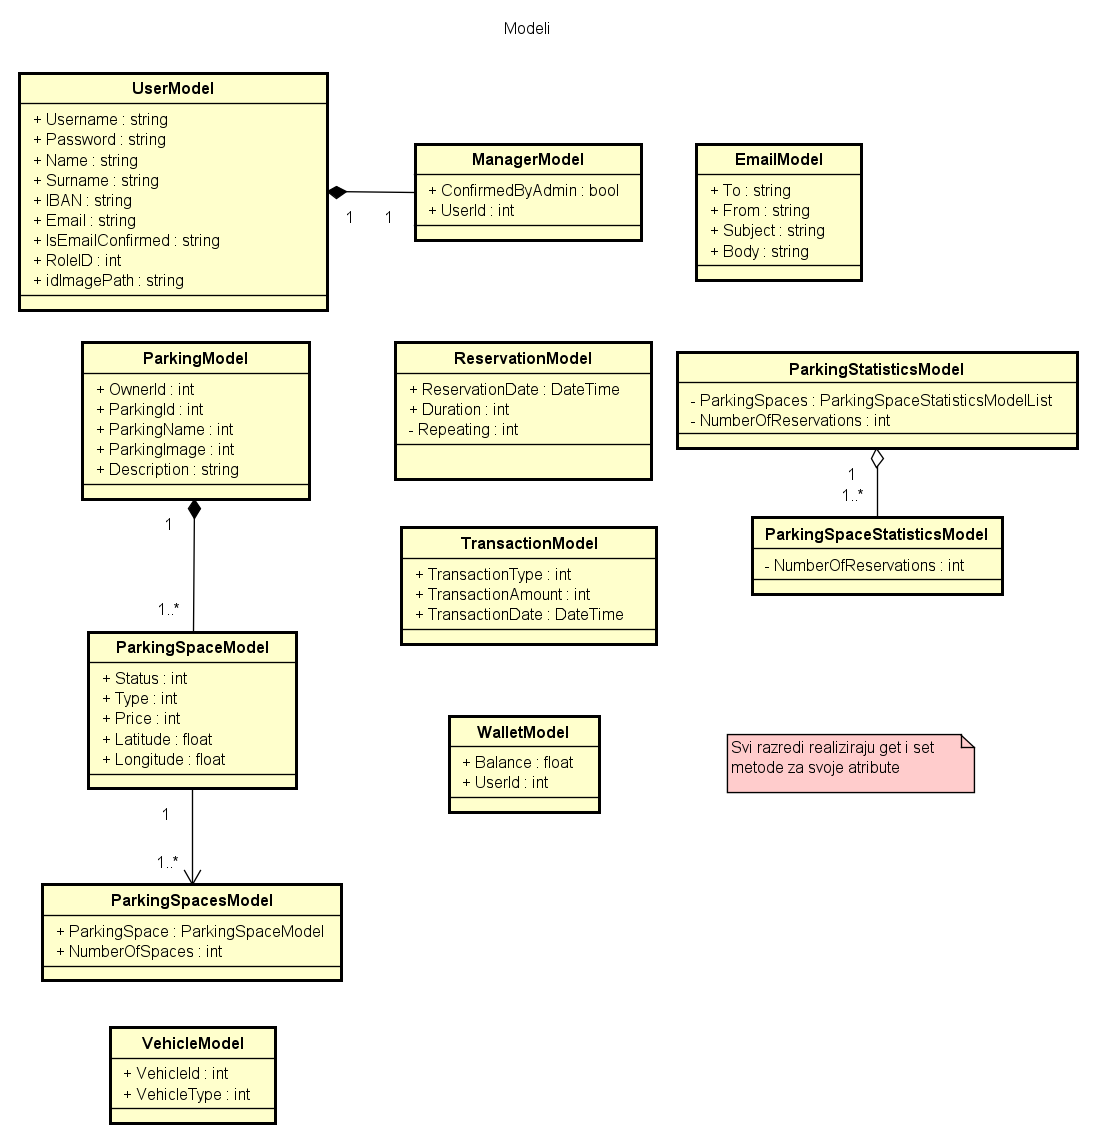
\includegraphics[width=\textwidth,keepaspectratio]{slike/progi_1.png}
				\caption{dio Models}
				\label{fig:models}
			\end{figure}
			\eject
			
			
			\begin{figure}[h]
				\centering
				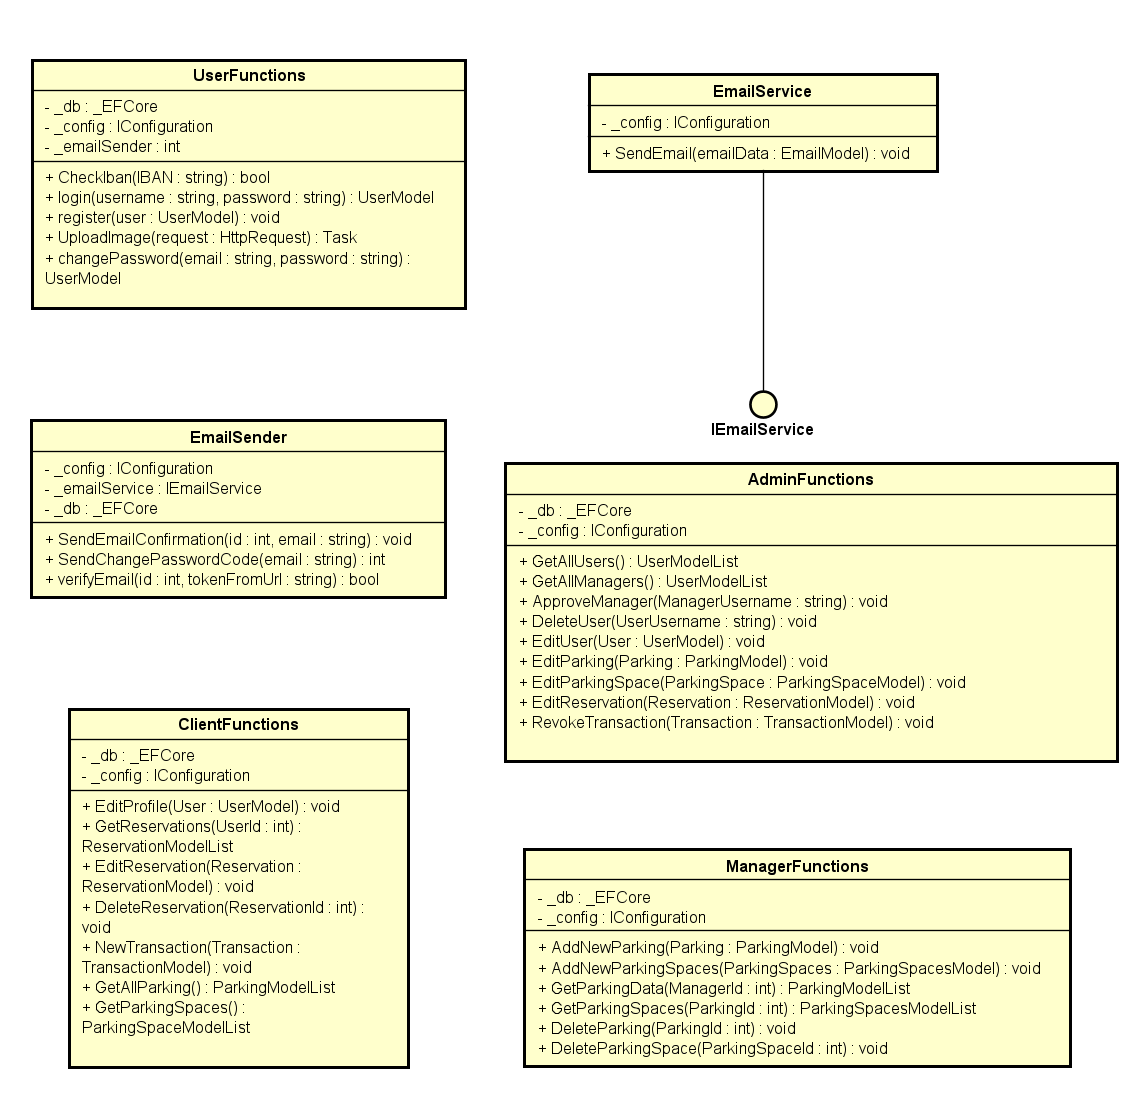
\includegraphics[width=\textwidth,keepaspectratio]{slike/progi3_1.png}
				\caption{dio Services}
				\label{fig:services}
			\end{figure}
			
			{U dijagramu razreda na slici \ref{fig:services} prikazani je dio servisa. Svi servisi kao svoj atribut, između ostalih, imaju instancu objekta \_EFCore koji predstavlja kontekst za bazu podataka i instancu IConfiguration objekta koji služi za dohvaćanje konstanti. Funkcije definirane u pojedinom razredu dohvaćaju, mijenjaju i dodaju podatke u bazu podataka i manipuliraju podacima koje vraćaju kontroleru koji šalje nazad do korisnika.}
			
			\begin{figure}[h]
				\centering
				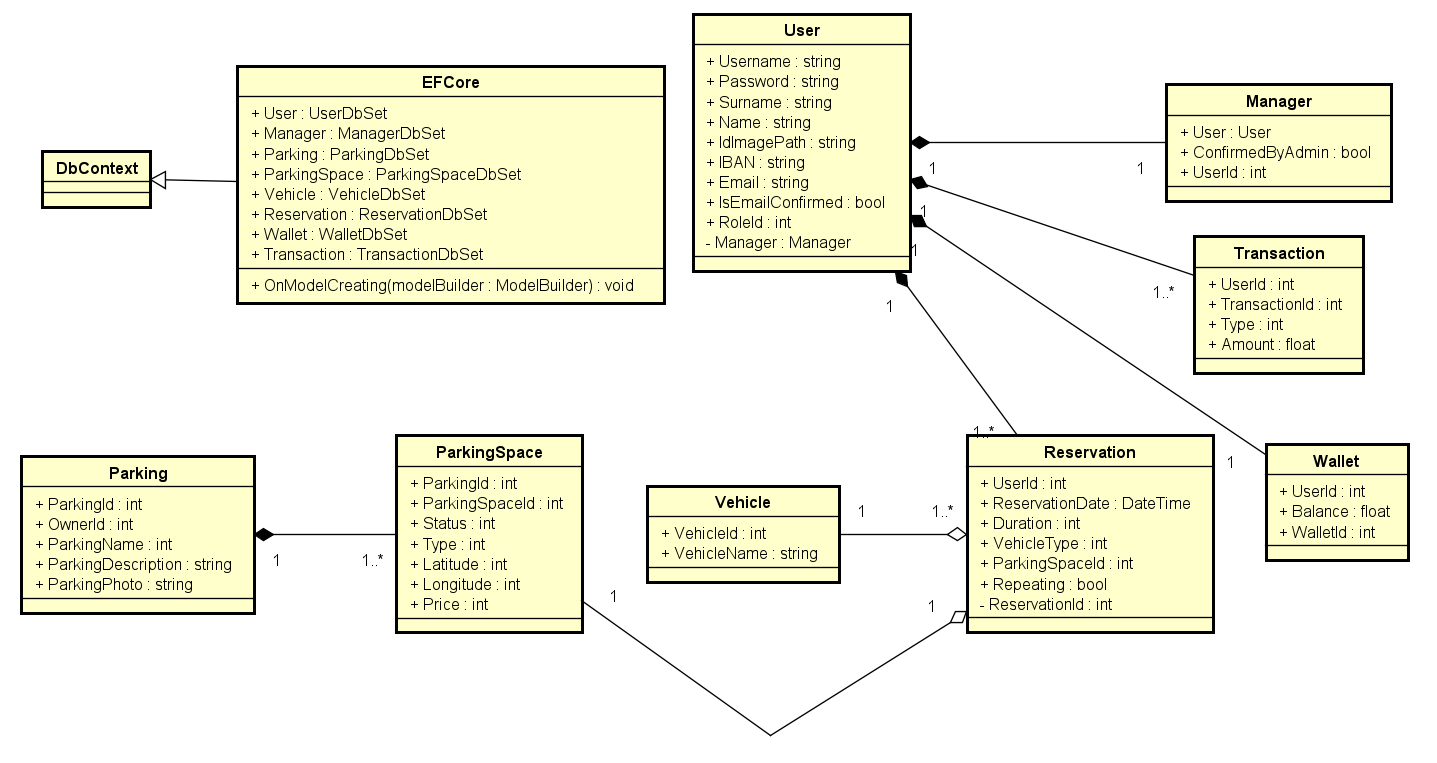
\includegraphics[width=\textwidth,keepaspectratio]{slike/progi2_1.png}
				\caption{Reprezentacija baze podataka}
				\label{fig:repr}
			\end{figure}
			
			\eject
			
			\pagebreak
			
			\section{Dijagram stanja}
			
			\textbf{\textit{dio 2. revizije}}\\
			
			\textit{Potrebno je priložiti dijagram stanja i opisati ga. Dovoljan je jedan dijagram stanja koji prikazuje \textbf{značajan dio funkcionalnosti} sustava. Na primjer, stanja korisničkog sučelja i tijek korištenja neke ključne funkcionalnosti jesu značajan dio sustava, a registracija i prijava nisu. }
			
			
			\eject 
			
			\section{Dijagram aktivnosti}
			
			\textbf{\textit{dio 2. revizije}}\\
			
			\textit{Potrebno je priložiti dijagram aktivnosti s pripadajućim opisom. Dijagram aktivnosti treba prikazivati značajan dio sustava.}
			
			\eject
			\section{Dijagram komponenti}
			
			\textbf{\textit{dio 2. revizije}}\\
			
			\textit{Potrebno je priložiti dijagram komponenti s pripadajućim opisom. Dijagram komponenti treba prikazivati strukturu cijele aplikacije.}
			
			
		\section{Dijagram razreda} 
			
			{ Na slikama su prikazani razredi („Class“) koji su korišteni za implementaciju backend-a. Na slici \ref{fig:controllers} su prikazani razredi koji nasljeđuju Controller razred. Sve funkcije implementirane u Controller razredu vraćaju IActionResult (podatke i odgovarajući kod). Također, sve funkcije ne komuniciraju direktno s bazom podataka nego pozivaju funkcije iz određenih servisa koji imaju implementiranu tu funkcionalnost. Funkcije u kontrolerima kao parametre primaju odgovarajući model. }
			
			\begin{figure}[h]
				\centering
				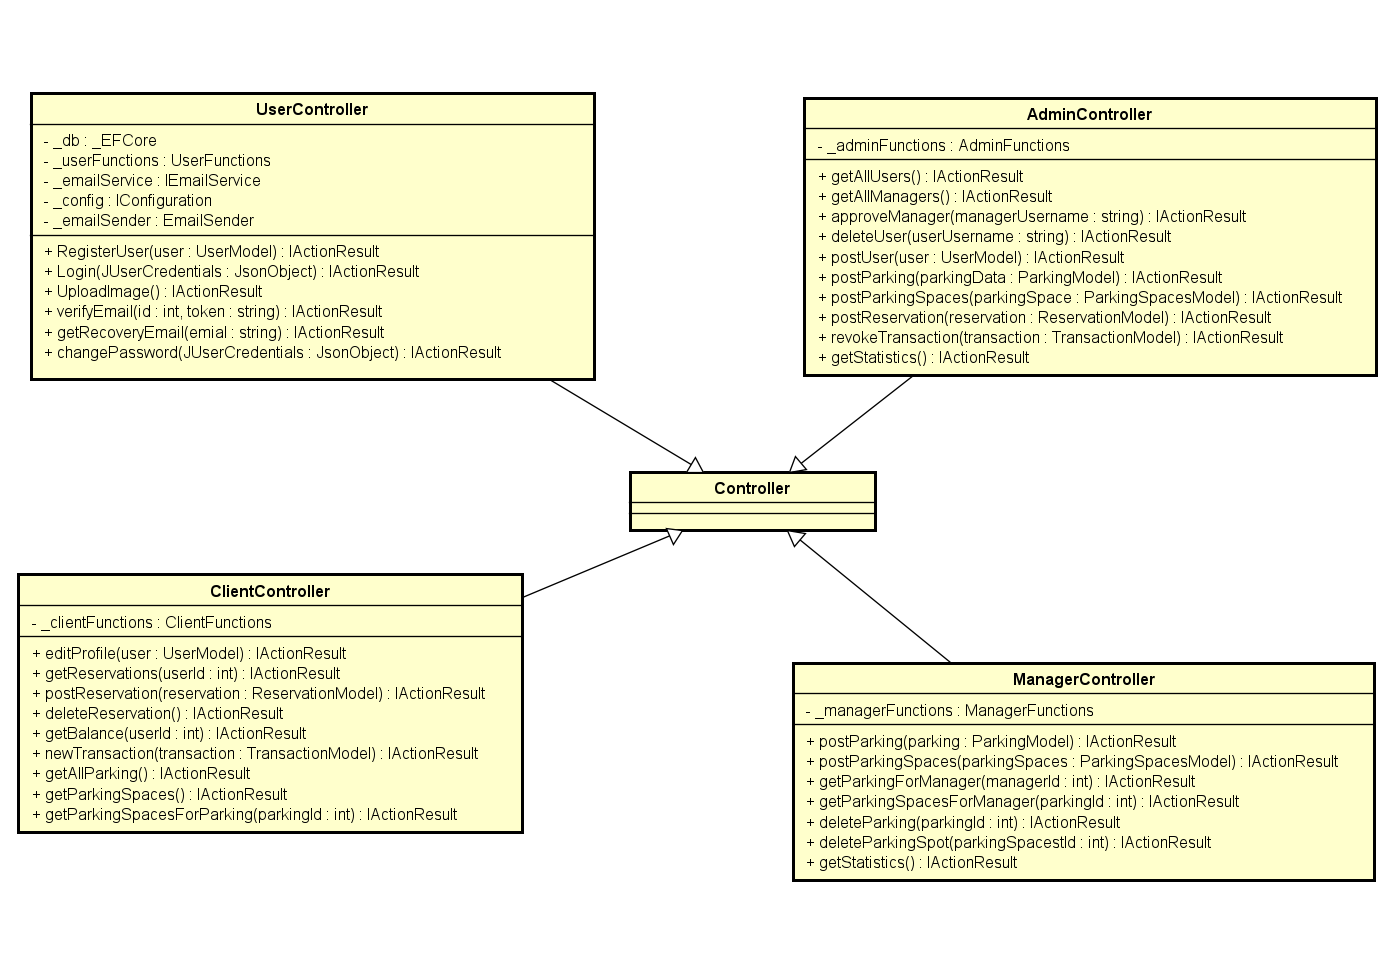
\includegraphics[width=\textwidth,keepaspectratio]{slike/progi4_1.png}
				\caption{dio Controllers}
				\label{fig:controllers}
			\end{figure}
			\pagebreak
			
			{Modeli razreda odražavaju strukturu baze podataka unutar aplikacije. Metode implementirane unutar tih razreda izravno komuniciraju s bazom podataka kako bi dobile tražene informacije. Razred User predstavlja generičnog korisnika aplikacije koji se može registrirati. Na taj razred referira se razred Manager (jer je svaki Manager ujedno i User).}
			
			\begin{figure}[h]
				\centering
				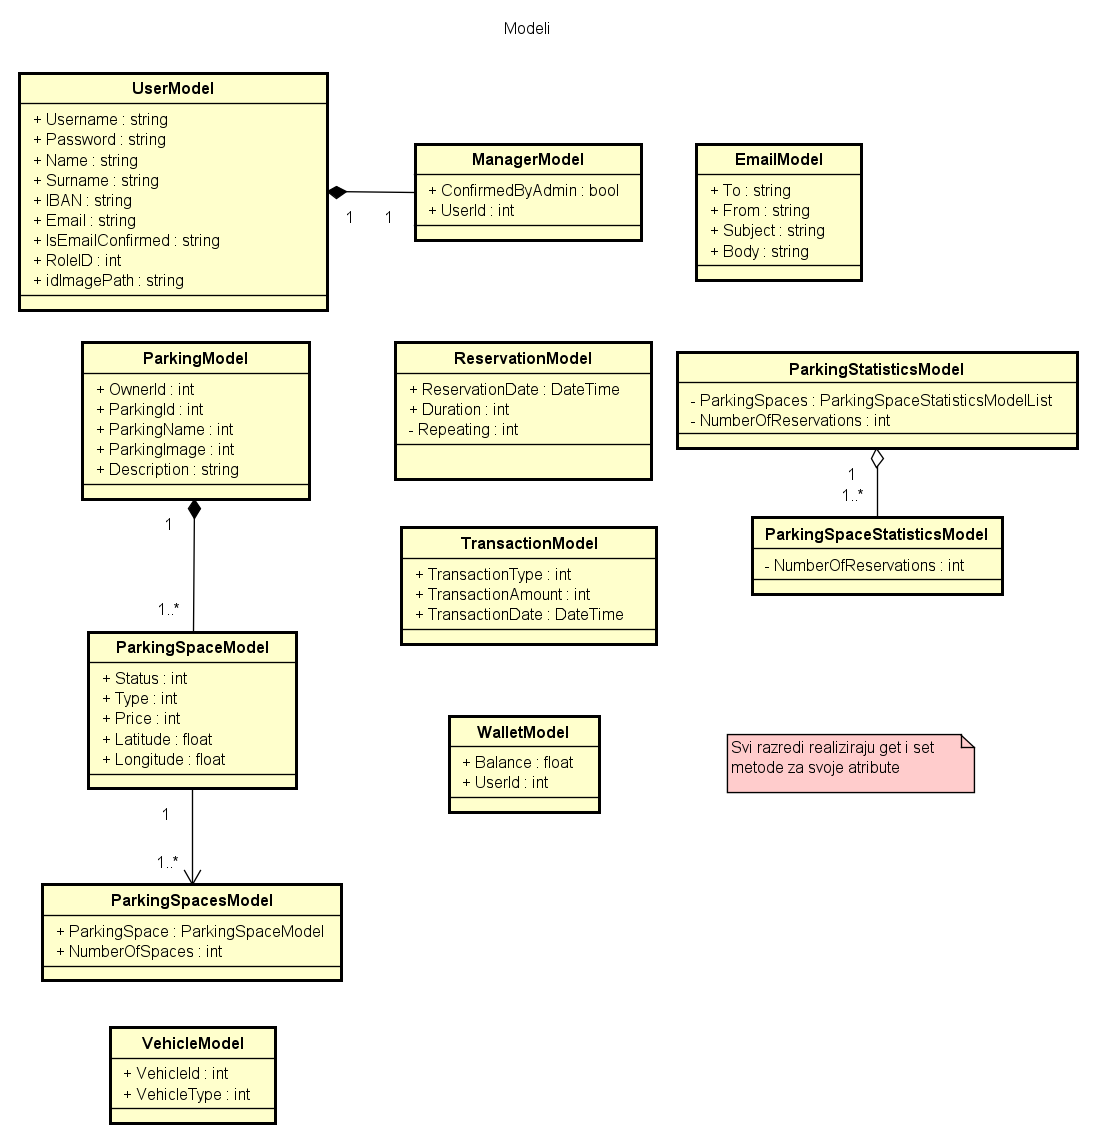
\includegraphics[width=\textwidth,keepaspectratio]{slike/progi_1.png}
				\caption{dio Models}
				\label{fig:models}
			\end{figure}
			\eject
		
			
			\begin{figure}[h]
				\centering
				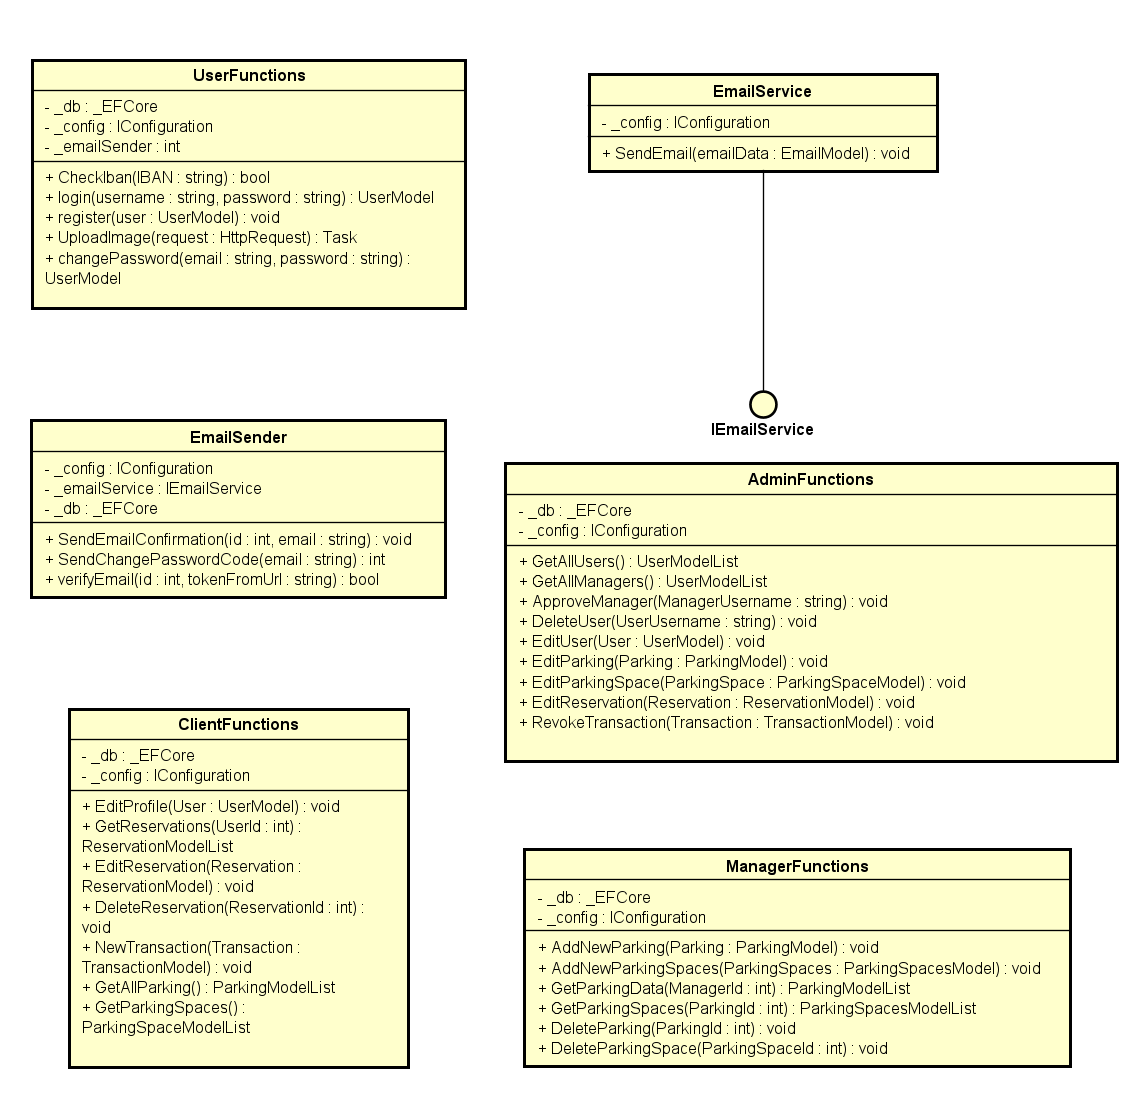
\includegraphics[width=\textwidth,keepaspectratio]{slike/progi3_1.png}
				\caption{dio Services}
				\label{fig:services}
			\end{figure}
			
			{U dijagramu razreda na slici \ref{fig:services} prikazani je dio servisa. Svi servisi kao svoj atribut, između ostalih, imaju instancu objekta \_EFCore koji predstavlja kontekst za bazu podataka i instancu IConfiguration objekta koji služi za dohvaćanje konstanti. Funkcije definirane u pojedinom razredu dohvaćaju, mijenjaju i dodaju podatke u bazu podataka i manipuliraju podacima koje vraćaju kontroleru koji šalje nazad do korisnika.}
			
			\begin{figure}[h]
				\centering
				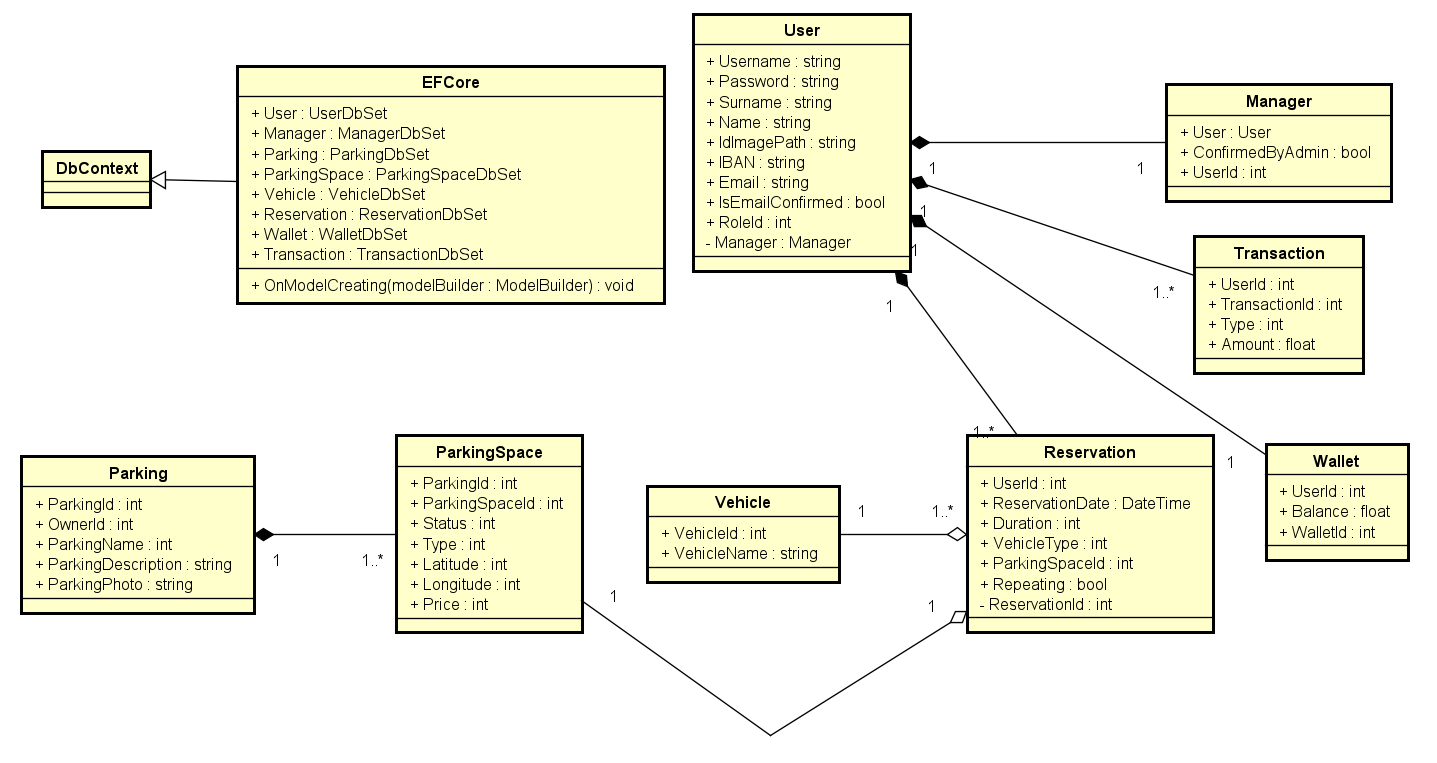
\includegraphics[width=\textwidth,keepaspectratio]{slike/progi2_1.png}
				\caption{Reprezentacija baze podataka}
				\label{fig:repr}
			\end{figure}
			
			\eject
			
			\pagebreak
		
		\section{Dijagram stanja}
			
			\textbf{\textit{dio 2. revizije}}\\
			
			\textit{Potrebno je priložiti dijagram stanja i opisati ga. Dovoljan je jedan dijagram stanja koji prikazuje \textbf{značajan dio funkcionalnosti} sustava. Na primjer, stanja korisničkog sučelja i tijek korištenja neke ključne funkcionalnosti jesu značajan dio sustava, a registracija i prijava nisu. }
			
			
			\eject 
		
		\section{Dijagram aktivnosti}
			
			\textbf{\textit{dio 2. revizije}}\\
			
			 \textit{Potrebno je priložiti dijagram aktivnosti s pripadajućim opisom. Dijagram aktivnosti treba prikazivati značajan dio sustava.}
			
			\eject
		\section{Dijagram komponenti}
		
			\textbf{\textit{dio 2. revizije}}\\
		
			 \textit{Potrebno je priložiti dijagram komponenti s pripadajućim opisom. Dijagram komponenti treba prikazivati strukturu cijele aplikacije.}